%! TEX root = /home/simon/Documents/Dagbok_MPPHS_2020-2021/main.tex
\subsection*{Tisdag 2020-08-11}

Kollade på en video som Thisplace lade upp på youtube som handlade om uncanny valley. I den visade han en graf på en kurvanpassning som några forskare hade gjort när dom undersökte fenomenet. Jag tyckte inte kurvanpassningen såg superövertygande ut, så jag gjorde min \href{https://github.com/SimonKvantdator/Uncanny-valley-data-analysis.git}{\color{blue}egen}. Först återskapade jag deras kurvanpassning, \cref{subfig:third_degree_curve_fit}. Sedan gjorde jag några egna, typ som \cref{subfig:first_degree_curve_fit}. Med Bayesian information criterion (BIC) som goodness-of-fit-metrik fick jag att \cref{subfig:third_degree_curve_fit} hade $\textrm{BIC} = 796.24$ och \cref{subfig:third_degree_curve_fit} hade $\textrm{BIC} = 794.98$, vilket är aningens bättre. Det finns liksom inte jättemycket bevis för att det är en \enquote{valley} där vid typ 50 mechano-humanness betyg.

\begin{figure}[ht]
    \centering
    \begin{subfigure}{.5\linewidth}
        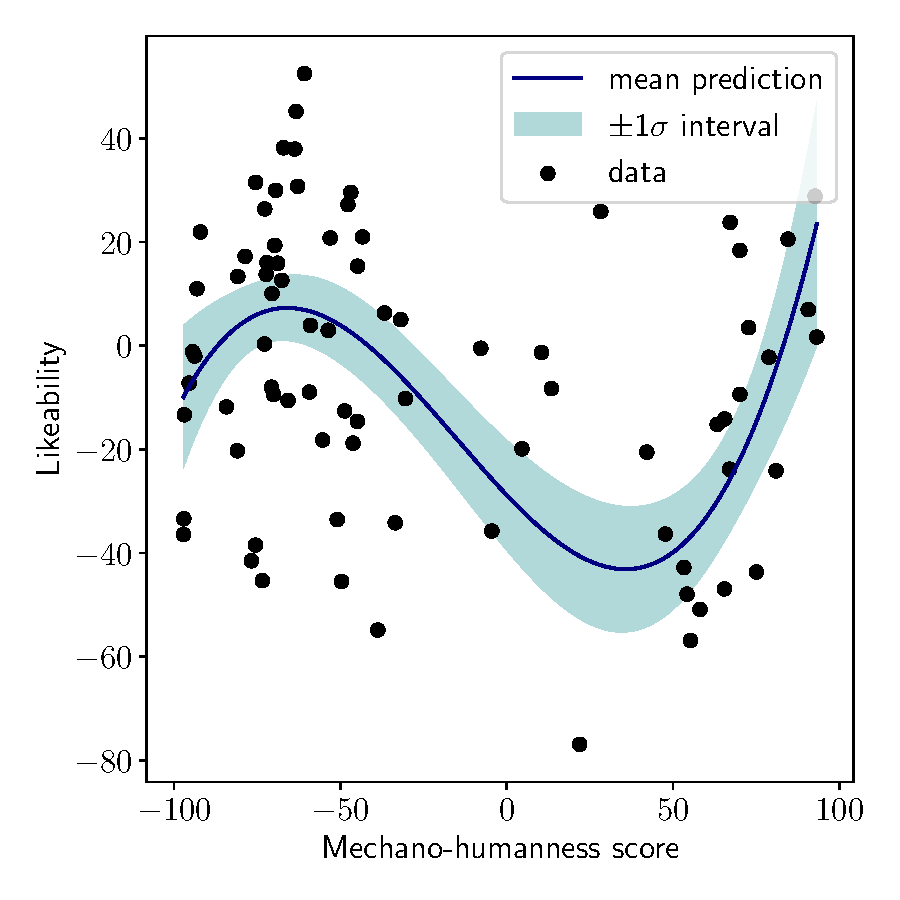
\includegraphics[width=\textwidth]{pics/third_degree_curve_fit.pdf}
        \caption{}
        \label{subfig:third_degree_curve_fit}
    \end{subfigure}%
    \begin{subfigure}{.5\linewidth}
        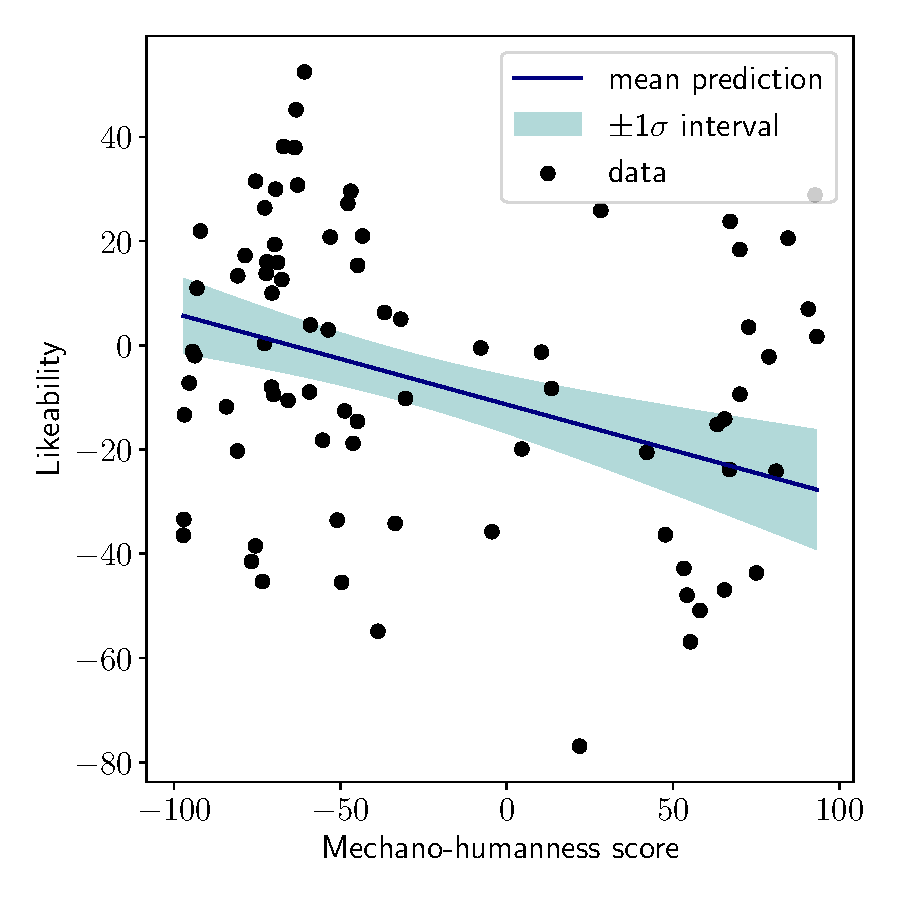
\includegraphics[width=\textwidth]{pics/first_degree_curve_fit.pdf}
        \caption{}
        \label{subfig:first_degree_curve_fit}
    \end{subfigure}
    \caption{}
\end{figure}

Mailade Jesse Agar \& visade vad jag ahde gjort, han verkade uppskatta det.

\bigskip

Jag har nu läst fram till kapitel 3 i algebraboken. Tror det kommer gå rätt bra att hinna läsa klart boken innan läsåret börjar. Planen för mastern är alltså fortfarande \cref{tab:course_plan}.

\begin{table}[H]
    \centering
    \caption{}
    \label{tab:course_plan}
    \begin{tabular}{l|l|l|}
         & Year 1 & Year 2 \\ \hline
        LP1 
        & \begin{tabular}[c]{@{}l@{}}
            \textcolor{compulsory}{Learning from data (C)}\\ \textcolor{compulsory}{Quantum mechanics (B)}\\ \textcolor{compulsory}{Experimental physics (A)}\\ Representation theory
        \end{tabular}
        & \begin{tabular}[c]{@{}l@{}} \textcolor{elective}{Standard model \& beyond (B)}\\ Integration theory\\ Commutative algebra?
        \end{tabular} \\ \hline
        LP2
        & \begin{tabular}[c]{@{}l@{}}
            \textcolor{compulsory_elective}{Symmetries (A)}\\ \textcolor{compulsory_elective}{Computational physics (D)}
        \end{tabular}
        & \begin{tabular}[c]{@{}l@{}}
            \textcolor{elective}{String theory (A)}\\
            Algebraic geometry\\
            Sannolikhetsteorins grunder?
        \end{tabular} \\ \hline
        LP3
        & \begin{tabular}[c]{@{}l@{}}
            \textcolor{elective}{Gravitation \& cosmology (A)}\\ Advanced differential calculus
        \end{tabular} &  \\ \hline
        LP4
        & \begin{tabular}[c]{@{}l@{}}
            \textcolor{elective}{Quantum field theory (B)}\\ Vetenskapshistoria (LA)\\ Complex analysis in several variables? (B?)
        \end{tabular} 
        & \begin{tabular}[c]{@{}l@{}}
            Distributionsteori?
        \end{tabular} \\ \hline
    \end{tabular}
\end{table}

Thomas Wernståhl mailade imorse om undervisning LP1, så nu e jag anmäld som räkneövningsledare och labbhandledare till TMV157, inledande matte för maskinarna(?). Lite oklart än sålänge om ngt av dom passen krockar med standardmodellen än, menmen.

\bigskip

Jag laddade även ner Termux, en app så jag kan köra en terminal i mobilen. Sen startade jag en SSH-server på min dator så att jag ska kunna logga in på datorn från mobilen. Jag gjorde såhär:
\begin{enumerate}
    \item installera servern med \texttt{sudo apt-get openssh-server}
    \item öppna http://192.168.1.254 i webbläsaren för att komma åt routern
    \item Verktyg $\blacktriangleright$ spel \& programdelning $\blacktriangleright$ Nytt spel eller program
    \item skapa \texttt{simons ssh} (Manuell inmatning av portmappningar), tryck nästa
    \item båda \texttt{Portområde} samt \texttt{Översätt till} ska vara 22, tryck lägg till
    \item Verktyg $\blacktriangleright$ spel \& programdelning $\blacktriangleright$ Tilldela ett spel eller ett program till en lokal nätverksenhet
\end{enumerate}


\subsection*{Lördag 2020-08-15}

Jag kom att tänka på en fråga igår, om jag hittar ett ställe på google reviews med $n = N$ reviews \& med medelbetyg $s = S$, vad är sannolikheten $p(s)$ för olika limes-medelbetyg när $n \to \infty$? Jag skrev ett pythonscript som svarar på den frågan \& körde scriptet på en McDonalds i nordstan med 216 reviews. I \cref{subfig:mcdonalds_nordstan_ratings} visas fördelningen av dom 216 reviews som fanns, \& i \cref{subfig:mcdonalds_nordstan_rating_probabilities_histogram} visas sannolikhetsfördelningen $p(s)$ av limes-medelbetyget.

\begin{figure}[ht]
    \centering
    \begin{subfigure}{.5\linewidth}
        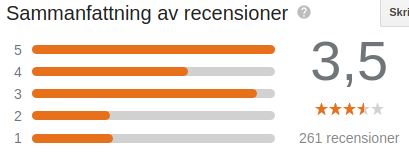
\includegraphics[width=\textwidth]{pics/mcdonalds_nordstan_ratings.png}
        \caption{}
        \label{subfig:mcdonalds_nordstan_ratings}
    \end{subfigure}%
    \begin{subfigure}{.5\linewidth}
        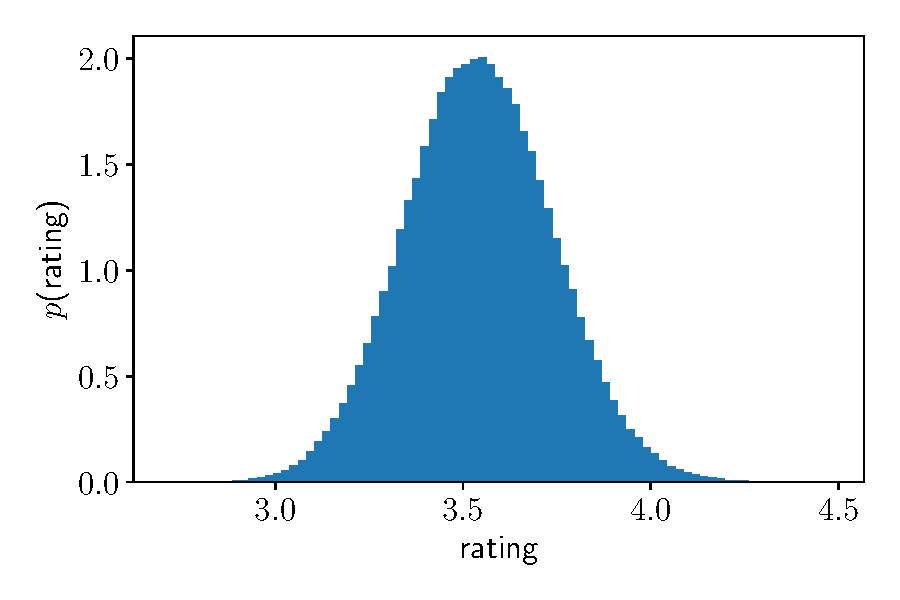
\includegraphics[width=\textwidth]{pics/mcdonalds_nordstan_rating_probabilities_histogram.pdf}
        \caption{}
        \label{subfig:mcdonalds_nordstan_rating_probabilities_histogram}
    \end{subfigure}
    \caption{}
\end{figure}

Det var relativt enkelt att ställa upp en modell: parametrarna var bara en sannolikhet $p_i$ för varje betyg. Det är skönt att för en gångs skull kunna sätta upp en modell som når alla möjliga tillstånd. Jag kunde återanvända den mesta av koden från uncanny valley-kurvanpassningen jag gjorde i början av veckan.

Jag funderar nu på om jag ska lägga resten av dagen på att få pale på google reviews-APIn så att jag kan automatisera datainsamlingen.

\bigskip

Igår var jag även ute med Elin \& åt på Moon Thai för att fira att hon fått jobb. Det var fett värd mat, borde gå dit igen!

\bigskip

Elin föreslog i morse att vi ska börja lyssna på Harry Potter-böckerna på morgonen istället för alla poddar vi lyssnar på atm. Jag tror det hade varit fett mysigt.


\subsection*{Måndag 2020-08-17}

Hade lite problem med Harry Potter-ljudboken jag laddade ner, metadatan var fel så min ljudboksuppspelare kunde inte sortera kapitlena rätt. Skrev ett pythonscript,
\begin{lstlisting}[language=python]
import os

for i in range(1, 10):
	os.system(f'id3v2 --track {i} CH0{i}*')

for i in range(10, 100):
	os.system(f'id3v2 --track {i} CH{i}*')
\end{lstlisting}
som åtgärdade detta bodgeigt men snabbt.


\subsection*{Onsdag 2020-08-19}

Hade möte med Wulcan \& Lärkäng imorse. Dom presenterade lite vad dom forskar på: typ residyströmmar (generaliserade envarreresidyer), generaliserad argumentsprincip, \& flervarrevarianten av algebrans fundamentalsats. Det lät fett intressant men båda var tveksamma till om dom visste om några kopplingar till fysiken. Anders Hellman sa ju när jag mailade honom att \enquote{Exjobbet ska vara relevant för din utbildning. Alltså ska du ställa dig frågan om du, med din specialisering inom MPPHS, är bäst lämpad för exjobbet som du funderar på. Mitt tips brukar vara att fundera på 2 kurser som du har läst på MPPHS som är relevanta för exjobbet. Annars är min tolkning av fysik väldigt brett (läran om naturen) och då brukar det finnas ingångar till de flesta exjobb.}

Kanske att Daniel Persson, David Witt Nyström, eller någon annan i komplexgänget vet några kopplingar till fysiken och att jag ändå kan göra för Wulcan eller Lärkäng? Jag får känna efter lite \& se vad som blir bäst.

Wulcan \& Lärkäng namedropade annars lite namn med folk som jag hade kunnat fråga om exjobb:
\begin{itemize}
    \item Hjalmar Rosengren
    \item Martin Hallnäs
    \item Robert Berman (förmodligen upptagen)
    \item David Witt Nyström
    \item M Ludmilla
    \item Simone
    \item Håkan Andreasson
    \item Thomas Bäckdahl.
\end{itemize}

\bigskip

Har fortfarande mitt projekt med Vim kvar. Kanske ska göra en pågående projekt-lista?
\begin{itemize}
    \item Lära mig lite Vim
    \item 
\end{itemize}

\bigskip

Blev även taggad på en bok som Forssén rekommenderade på LFD-kurshemsidan, \enquote{Information Theory, Inference, and Learning Algorithms} av David J.C. MacKay. Lade till den i vill läsa-listan på goodreads.

\bigskip

Vi testar lite mattekommandon:
\begin{align}
    \transpose{A}
    \quad
    \complement{A}
    \quad
    \conjugate{A}
    \quad
    \hermitianconjugate{A}
    \quad
    \order{x^2}
\end{align}


\subsection*{Torsdag 2020-08-20}

Hade möte med dom andra rövningsledarna imorse. Det kommer bli asbra. Vi turas om om att räkna \enquote{på tavlan}, jag räknar första passet. Det enda vi behöver klura ut är hur man skapar break out rooms för att hjälpa folk enskilt. Jag tänkte även att vi löser demouppgifterna i ett \href{https://www.overleaf.com/read/bkttgyjvnqbx}{\color{blue}Overleafdokument} som man kan länka till på Canvas.


\subsection*{Måndag 2020-08-24}

Jag borde börja med att maila David Witt Nyström om exjobb. Som Elin sa borde jag nog inte hänga upp mig på att ha just Wulcan eller Lärkäng som handledare, \& dom nämnde att David kanske har bättre koll på fysiken. Borde ha som mål att formulera ett mail idag tror jag.

Jag mailade honom men han har inte svarat än, han svarar säkert imorgon.

\bigskip

Gabriele skrev på kurshemsidan för standardmodellen följande:
\begin{figure}[H]
    \centering
    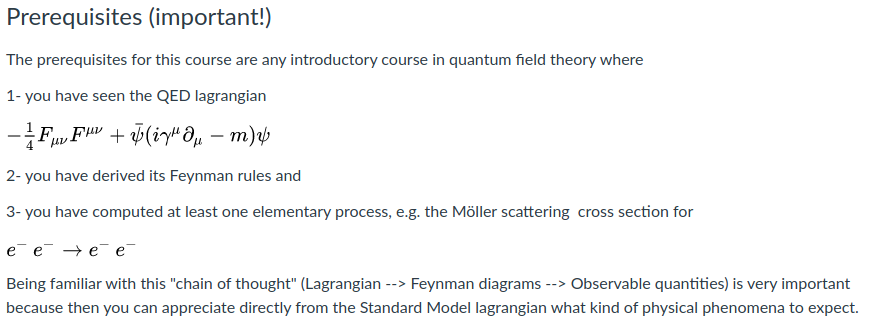
\includegraphics[width=1.0\textwidth]{pics/standard_model_prerequisites.png}
\end{figure}
Jag känner ju faktiskt inte spontant att jag har koll på det, så kanske borde repetera lite... Kanske är bra för mig att jag omtenterar subben nu ändå.


\subsection*{Torsdag 2020-08-27}

Elektronens massa är \SI{511.0}{\kilo \electronvolt\per \clight^2}.

Gjorde omtentan i subben idag. Kan ha gått hur som.


\subsection*{Fredag 2020-08-28}

$x \in \interval[open left]{-\infty}{0}$.

Hade möte med Ville \& Rövningsledarna imorse, tror det kommer fungera helt OK med rövningar \& sånt. Vi kommer ha ett zoomrum till föreläsningar \& rövningar \& sen ett zoomrum var för hjälp med uppgifter \& matlabhjälp.

